\documentclass[../main.tex]{subfiles}

\begin{document}

\newpage
{\LARGE\textbf{\faIcon{dice} XPixel Metaverse}}

%##################################################################################################
\begin{figure}[h]
    \vspace{1cm}
    \begin{center}
        %\fbox{\rule{0pt}{2.5in} \rule{0.9\linewidth}{0pt}}
        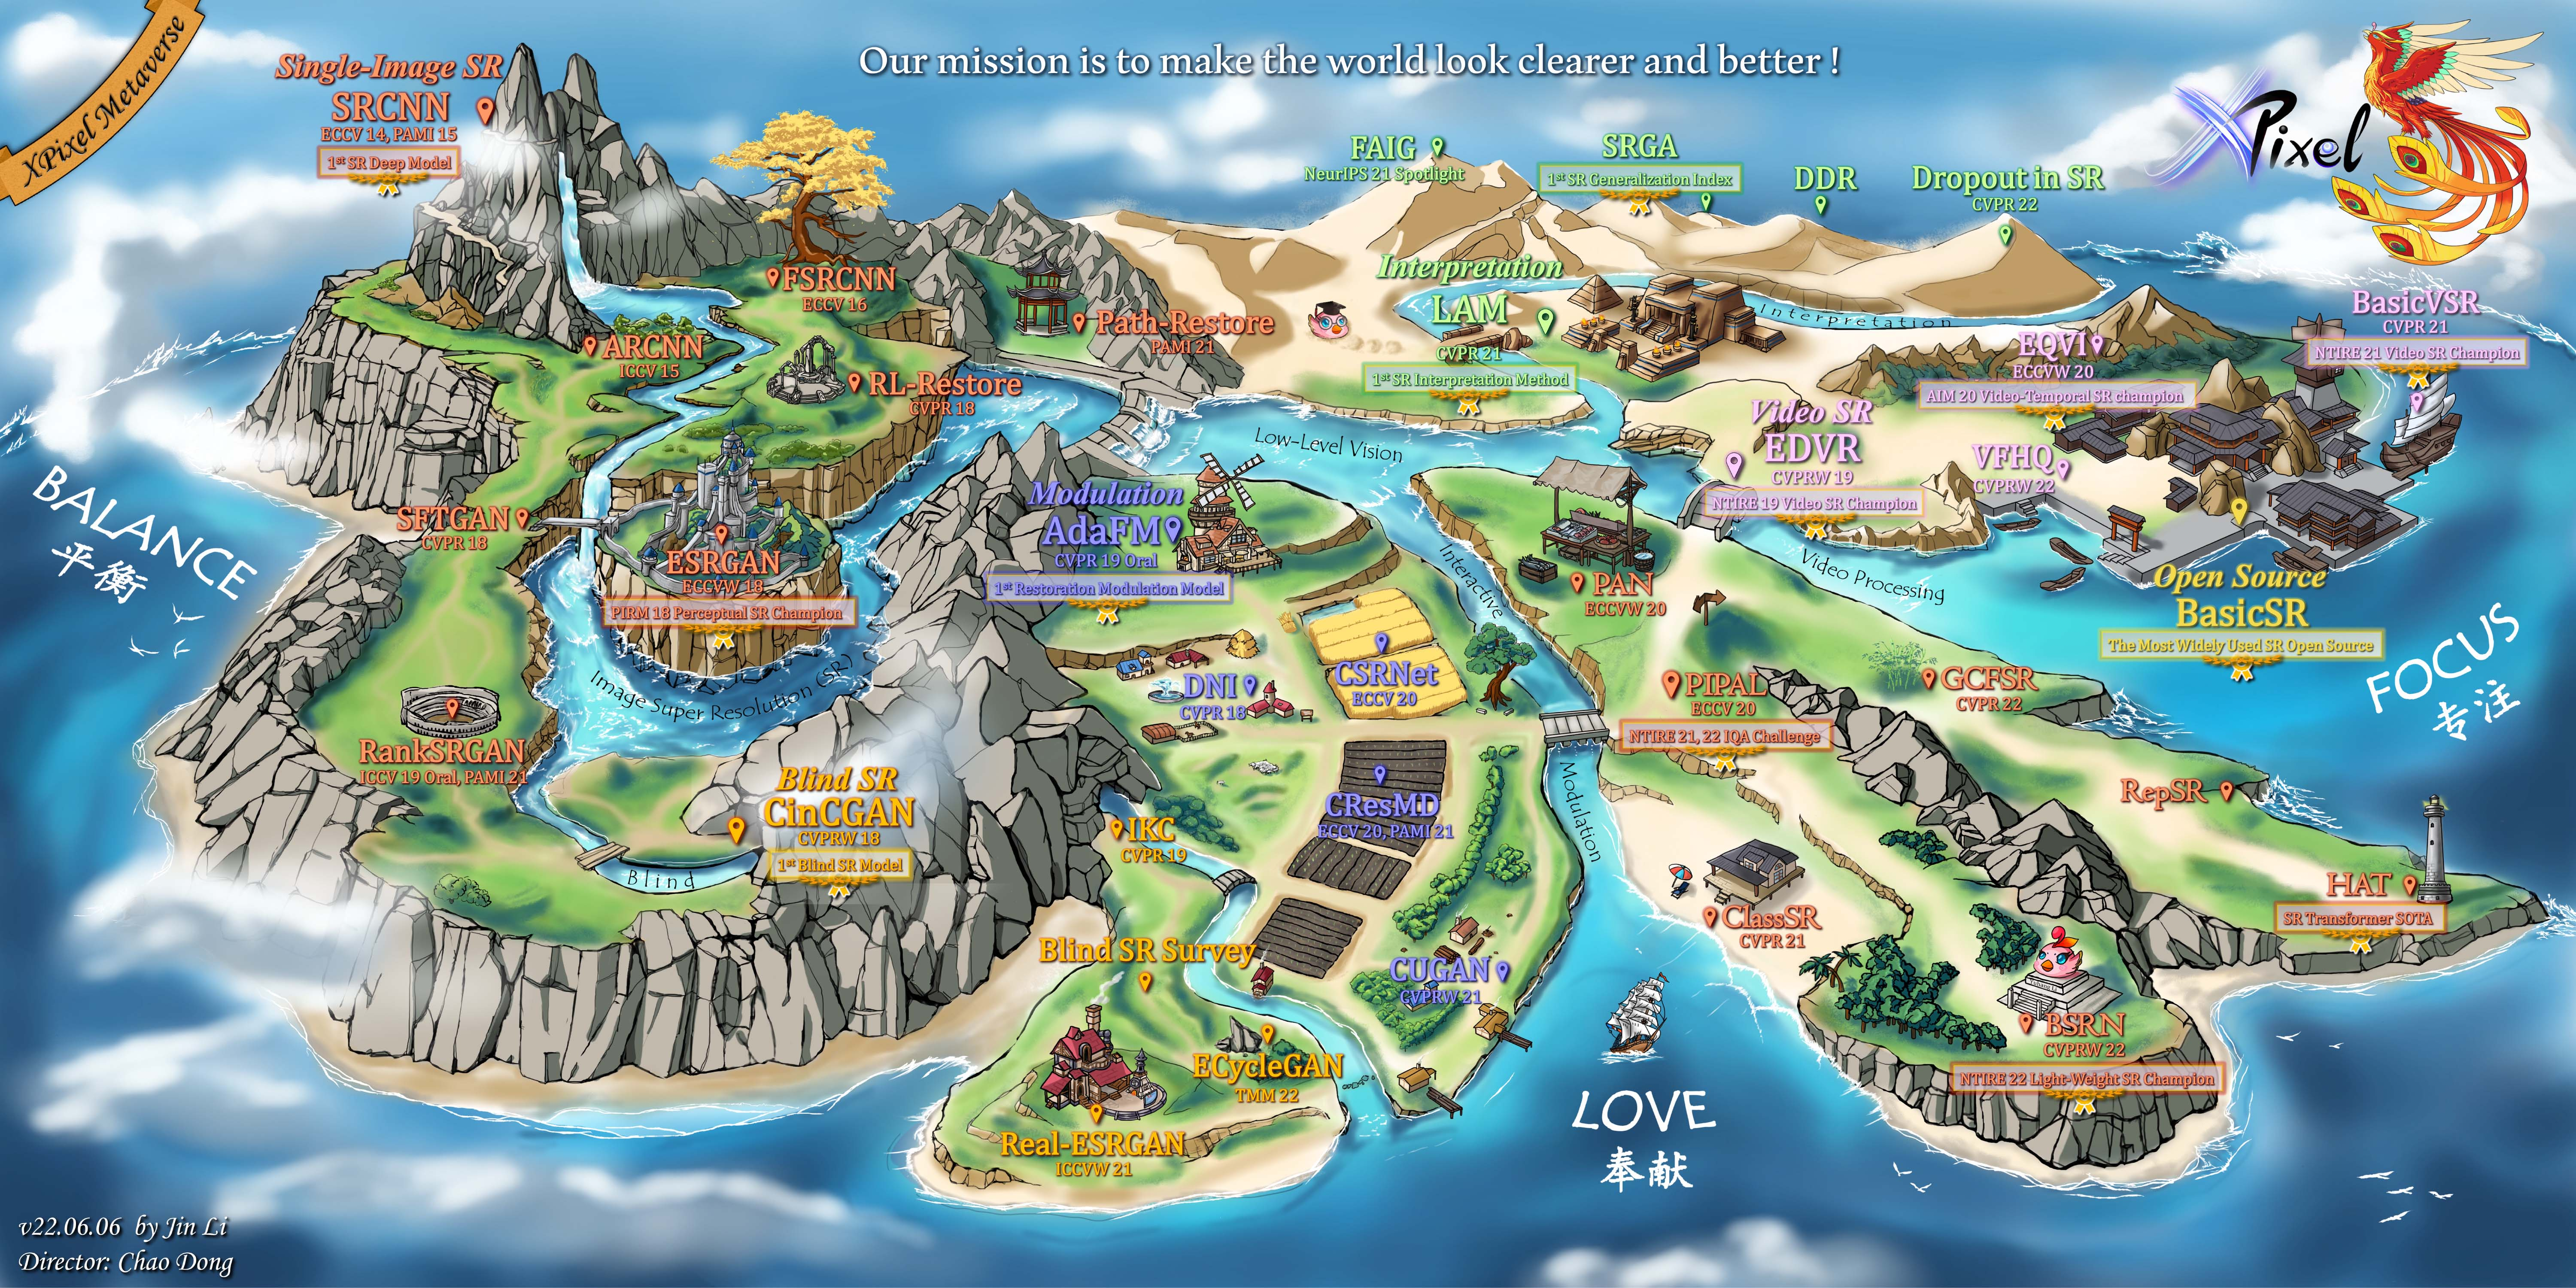
\includegraphics[width=\linewidth]{figures/XPixelMetaverse_small.jpg}
        \vspace{-0.7cm}
        \caption{XPixel 的元宇宙。你可以在\href{https://xpixel.group/2022/06/06/poster.html}{官网}查看更高清的版本。}
    \end{center}
    %\vspace{-0.6cm}
\end{figure}
%##################################################################################################

XPixel Metaverse 是 XPixel Group (官网:\url{https://xpixel.group/}) 集体智慧的结晶,它体现了 XPixel 所有成员对科研的坚持,对艺术的追求,对生活的热爱,和对世界的责任。
下面就请跟随文字向导,一起来巡游 XPixel 的历史和现在。

{\large\textbf{设计理念}}

为了完整而有特色地展示 XPixel Group 的各项科研成果,我们采用了“地图”的形式,通过山川、河流、建筑等元素,自然地将一项项科研成果与之对应,最终构成了 XPixel Metaverse。目前地图的大陆被三片海洋包围,中间的大陆则遍布 XPixel 从2014年到2022年来经典的科研成果,完美地将科技和艺术结合在了一起。

\textbf{海洋}

海洋以 XPixel 的组内文化:Love(奉献)、Focus(专注)、Balance(平衡)命名,象征着大陆上众多科研成果是在这种优秀的文化中孕育而成。而大陆的河流最终流入这三片汪洋之中,又象征着小组的工作成果最后又回归并加强了这种科研文化。

\textbf{大陆}

贯彻大陆的河流由左上角的高山发源,以此山代表深度学习超分辨率的开山之作 SRCNN,象征着这项工作重若泰山的源头意义。由此发源的河流上段命名为 Image Super Resolution(SR),此段周围的建筑与地形均是传统单图像超分的重要成果。同时在上段出现了最早的支流 Blind,象征着图像盲超分这一分支领域的出现。

顺主流而下到达一处大坝,大陆地形由高地形转为海拔更低更平坦的地形,象征着 XPixel 在早期工作的基础上,随着更多优秀同学的加入,科研工作的开展比以往更加顺利。在大坝下方形成的名为 Low-Level Vision 的湖泊分出三条河流,分别是:
\begin{itemize}
    \item 象征交互式可调节复原的:Interactive Modulation
    \item 象征超分网络可解释性的:Interpretation
    \item 象征视频处理和复原的:Video Processing
\end{itemize}

Interpretation 所流经的地图上方,其沙漠地貌与其他地方产生了强烈反差。这是因为底层视觉可解释性领域的工作非常稀少,且进展尤为不易,所以地貌较其他领域更加严酷。而这份不易对应的,是隐藏在沙漠背后未被探索的广袤空间。

在大陆的沿海处有一片码头区域,是超分领域最大的开源代码库 BasicSR。这是 XPixel 科研工作的重要载体和精华所在,同时也在国际上获得了广泛的使用与认可,与码头的作用高度契合。

\textbf{文字介绍及其他元素}

地图的左上角是作品的名称:XPixel Metaverse。地图正上方是 XPixel 的使命愿景:\textbf{Our mission is to make the world look clearer and better!} 地图右上角是 XPixel 的 logo,地图中沙漠和沿海的两处小凤凰是 XPixel 的吉祥物。

大陆上各个地形、建筑均以 XPixel 的科研成果命名,并添加文字介绍。文字介绍最多四行,从上到下:

\begin{itemize}
    \item 某领域的开创性成果,以斜体标明该新领域
    \item 工作的简称
    \item 工作发表的期刊及年份
    \item 工作的荣誉在最下方特别标明
\end{itemize}

同时为了能更轻松地辨识各个领域的成果,各领域成果均以地图右上角XPixel的Logo图案中的一个颜色进行着色。

\vspace{0.5cm}
XPixel Metaverse 承载着我们的历史,也呼唤着美好的未来!愿世界各地优秀的学者与我们一起,让世界变得更清晰,更美好!

\end{document}
